\documentclass[dvipsnames]{article}
\usepackage[english]{babel}
\usepackage{multirow}
\usepackage[letterpaper,top=2cm,bottom=2cm,left=3cm,right=3cm,marginparwidth=1.75cm]{geometry}
\usepackage{amsmath}
\usepackage{graphicx}
\usepackage{minted}
\usepackage{amsthm}
\usepackage{mathtools}
\usepackage[colorlinks=true, allcolors=blue]{hyperref}
\usepackage{fancyhdr}
\usepackage{enumerate}
\usepackage{tikz-cd}
\usepackage{mdframed}

\newmintinline[java]{java}{}

\usepackage{tikz}
\usetikzlibrary{shapes}
\usetikzlibrary{arrows}

\tikzset{
  treenode/.style = {align=center, inner sep=0pt, text centered,
    font=\sffamily},
  avl_node/.style = {treenode, circle, black, draw=black,
    text width=1.5em, very thick},% arbre rouge noir, noeud rouge
  black_node/.style = {treenode, circle, white, font=\sffamily\bfseries, draw=black,
    fill=black, text width=1.5em},% arbre rouge noir, noeud noir
  red_node/.style = {treenode, circle, red, draw=red,
    text width=1.5em, very thick},% arbre rouge noir, noeud rouge
  nil_leaf/.style = {treenode, rectangle, draw=black, fill=black,
    minimum width=0.3em, minimum height=0.3em}% arbre rouge noir, nil
}

\begin{document}
\section*{Week 11. Problem set (solutions by \textcolor{blue}{Karim Khabibrakhmanov})}

\thispagestyle{fancy}
\lhead{Karim Khabibrakhmanov (\texttt{k.khabibrakhmanov@innopolis.university}), group B24-DSAI-05}

\begin{enumerate}

  \item Run Prim-Jarn\'ik algorithm~\cite[\S 21.2]{Cormen2022} on the following graph $\mathcal{G}$, starting at vertex $S$,
  and answer the questions below.
  
  \begin{center}
  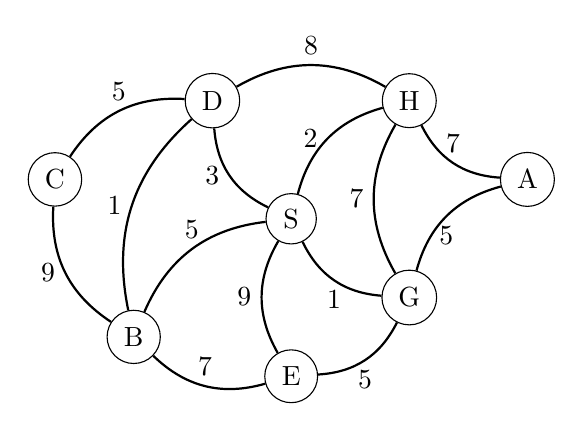
\begin{tikzpicture}
  
  \tikzset{vertex/.style = {shape=circle,draw,minimum size=1.5em}}
  \tikzset{edge/.style = {-,> = latex',thick}}
  % vertices
  \node[vertex] (a) at  (4,4)   {A};
  \node[vertex] (b) at  (-1,2)   {B};
  \node[vertex] (c) at  (-2,4)   {C};
  \node[vertex] (d) at  (0,5)   {D};
  \node[vertex] (e) at  (1,1.5)  {E};
  \node[vertex] (f) at  (1,3.5)  {S};
  \node[vertex] (g) at  (2.5,2.5) {G};
  \node[vertex] (h) at  (2.5,5)  {H};
  %edges
  \draw[edge] (h) to[bend right, above] node {$7$} (a);
  \draw[edge] (b) to[bend left,  left]  node {$9$} (c);
  \draw[edge] (b) to[bend left,  left] node {$1$} (d);
  \draw[edge] (c) to[bend left,  above] node {$5$} (d);
  \draw[edge] (d) to[bend left,  above] node {$8$} (h);
  \draw[edge] (e) to[bend left,  above] node {$7$} (b);
  \draw[edge] (f) to[bend left,  left] node {$3$} (d);
  \draw[edge] (f) to[bend right, left] node {$9$} (e);
  \draw[edge] (g) to[bend left,  below]  node {$5$} (e);
  \draw[edge] (g) to[bend left,  below]  node {$1$} (f);
  \draw[edge] (g) to[bend left,  left] node {$7$} (h);
  \draw[edge] (a) to[bend right, below] node {$5$} (g);
  \draw[edge] (f) to[bend left,  left] node {$2$} (h);
  \draw[edge] (b) to[bend left,  above] node {$5$} (f);
  \end{tikzpicture}
  \end{center}

  \begin{enumerate}
    \item Draw a minimum spanning tree of the graph $\mathcal{G}$.

    \color{blue}
    \textbf{Answer:}
    \begin{center}
      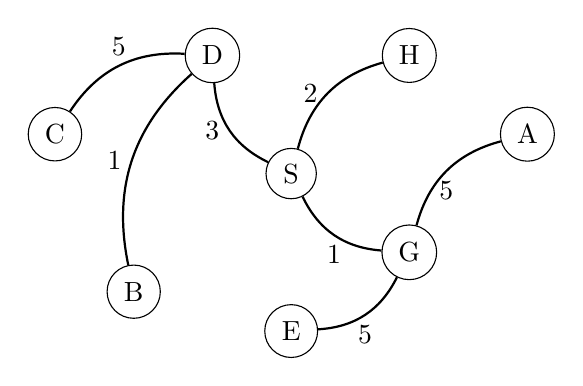
\begin{tikzpicture}
      
      \tikzset{vertex/.style = {shape=circle,draw,minimum size=1.5em}}
      \tikzset{edge/.style = {-,> = latex',thick}}
      % vertices
      \node[vertex] (a) at  (4,4)   {A};
      \node[vertex] (b) at  (-1,2)   {B};
      \node[vertex] (c) at  (-2,4)   {C};
      \node[vertex] (d) at  (0,5)   {D};
      \node[vertex] (e) at  (1,1.5)  {E};
      \node[vertex] (f) at  (1,3.5)  {S};
      \node[vertex] (g) at  (2.5,2.5) {G};
      \node[vertex] (h) at  (2.5,5)  {H};
      %edges
      \draw[edge] (g) to[bend left,  below]  node {$1$} (f);
      \draw[edge] (a) to[bend right, below] node {$5$} (g);
      \draw[edge] (c) to[bend left,  above] node {$5$} (d);
      \draw[edge] (f) to[bend left,  left] node {$3$} (d);
      \draw[edge] (f) to[bend left,  left] node {$2$} (h);
      \draw[edge] (b) to[bend left,  left] node {$1$} (d);
      \draw[edge] (g) to[bend left,  below]  node {$5$} (e);
      \end{tikzpicture}
      \end{center}
    \color{black}

    \item Is the minimum spaning tree for graph $\mathcal{G}$ unique?

    \color{blue}
    \textbf{Answer:}\\
    Yes, because when executing the \textbf{Prim-Jarn\'ik algorithm}, there was no ambiguity in the choice of edges. All edges with the same weights were either uniquely added to the \textbf{MST}, or uniquely excluded:\\
    \hspace*{5mm} 
        \textbf{1)} The vertex \textbf{G} has two edges with a weight of 5, and they are both included in the\\\hspace*{5mm} spanning tree.\\\hspace*{5mm}
        \textbf{2)} The vertex \textbf{H} has two edges with weight 7, and they are both not included in the\\\hspace*{5mm} spanning tree.
        
    \color{black}

    \item
    Assuming that the algorithm is using Binary Heap implementation~\cite[\S 6]{Cormen2022} of a priority queue,
    show the state of the priority queue after each iteration of the algorithm (i.e. after adding each new vertex to the MST).
    The graph contains 8 vertices, which means that your solution must provide 8 states of the Binary heap.
    Each heap state must be represented as an array.

    For example, a binary min-heap containing key-value pairs $\langle 3, a\rangle, \langle 2, b\rangle, \langle 1, c\rangle, \langle 4, d\rangle$
    may be represented as follows:

    \begin{center}
    \begin{tabular}{|c|c|c|c|}
      \hline \makebox[\widthof{000}][c]{$1, c$}
          & \makebox[\widthof{000}][c]{$3, a$}
          & \makebox[\widthof{000}][c]{$2, b$}
          & \makebox[\widthof{000}][c]{$4, d$} \\
      \hline
    \end{tabular}
    \end{center}

    \color{blue}
    \textbf{Answer:}\\
    1.
    \begin{tabular}{|c|c|c|c|c|}
      \hline \makebox[\widthof{000}][c]{$1, G$}
          & \makebox[\widthof{000}][c]{$2, H$}
          & \makebox[\widthof{000}][c]{$3, D$}
          & \makebox[\widthof{000}][c]{$5, B$}
          & \makebox[\widthof{000}][c]{$9, E$}\\
      \hline
    \end{tabular}\\
    2.
    \begin{tabular}{|c|c|c|c|c|}
      \hline \makebox[\widthof{000}][c]{$2, H$}
          & \makebox[\widthof{000}][c]{$5, B$}
          & \makebox[\widthof{000}][c]{$3, D$}
          & \makebox[\widthof{000}][c]{$5, E$}
          & \makebox[\widthof{000}][c]{$5, A$}\\
      \hline
    \end{tabular}\\
    3.
    \begin{tabular}{|c|c|c|c|}
      \hline \makebox[\widthof{000}][c]{$3, D$}
          & \makebox[\widthof{000}][c]{$5, B$}
          & \makebox[\widthof{000}][c]{$5, A$}
          & \makebox[\widthof{000}][c]{$5, E$}\\
      \hline
    \end{tabular}\\
    4.
    \begin{tabular}{|c|c|c|c|}
      \hline \makebox[\widthof{000}][c]{$1, B$}
          & \makebox[\widthof{000}][c]{$5, E$}
          & \makebox[\widthof{000}][c]{$5, A$}
          & \makebox[\widthof{000}][c]{$5, C$}\\
      \hline
    \end{tabular}\\
    5.
    \begin{tabular}{|c|c|c|c|}
      \hline \makebox[\widthof{000}][c]{$5, C$}
          & \makebox[\widthof{000}][c]{$5, E$}
          & \makebox[\widthof{000}][c]{$5, A$}\\
      \hline
    \end{tabular}\\
    6.
    \begin{tabular}{|c|c|c|c|}
      \hline \makebox[\widthof{000}][c]{$5, A$}
          & \makebox[\widthof{000}][c]{$5, E$}\\
      \hline
    \end{tabular}\\
    7.
    \begin{tabular}{|c|c|c|c|}
      \hline \makebox[\widthof{000}][c]{$5, E$}\\
      \hline
    \end{tabular}\\
    8.
    \begin{tabular}{|c|c|c|c|}
      \hline \makebox[\widthof{000}][c]{$$}\\
      \hline
    \end{tabular}\\
    \color{black}
  \end{enumerate}
  \item Suppose that $T$ is the minimum spaning tree for graph $\mathcal{G}$.
  How difficult is it to update the minimum spanning tree after adding a new vertex and its incident edges to $\mathcal{G}$.
  
  \begin{enumerate}
    \item Describe your algorithm (write pseudocode).

    \color{blue}
    \textbf{Answer:}
\begin{minted}[linenos, escapeinside=||, breaklines]{cpp}
UpdateSpanningTree(old T, new vertex, vector<Edge*> allAdjToVertex):
  T->addVertex(vertex)
  
  for (Edge* edge : allAdjToVertex):
    T->addEdge(edge)
    
  T = Kruskal-Algorithm(T)
  return T
\end{minted}
    \color{black}

    \item Provide the asymptotic time complexity for your algorithm.

    \color{blue}
    \textbf{Answer:} $\Theta(|V|\cdot \log(|V|))$
    \color{black}

    \item Justify the asymptotic time complexity (1--3 sentences).

    \color{blue}
    \textbf{Justification:}\\
    Adding a vertex takes $\Theta(1)$. Adding all sides will take $\Theta(|V|-1)$ in the worst case, if the new vertex is connected to each old one. The most expensive is the Kruskal's algorithm, which takes $\Theta(|V|\cdot \log(|V|))$, but since the maximum number of edges in the algorithm is the old $|V| -1$ and the new ones added in the worst case $|V| - 1$ give us $\Theta((2\cdot |V|-2)\cdot \log(|V|)) \approx \Theta(|V|\cdot \log(|V|))$. Therefore, $\Theta(1 + |V| - 1+|V|\cdot \log(|V|)) \approx \Theta(|V|\cdot \log(|V|))$
    \color{black}
  \end{enumerate}

  \clearpage
  \item Suppose that all edge weights in a graph are \emph{real numbers} uniformly distributed in the range from $0$ to $k$.

  \begin{enumerate}
    \item Which of the MST algorithms, Kruskal's or Prim's (possibly with minor modifications) can run faster on such a graph?

    \color{blue}
    \textbf{Answer:} Kruskal's algorithm, because we can implement sorting of the sides' weights in linear time. This gives us an advantage over Prim's algorithm.
    
    \color{black}

    \item Which modification is required to make the algorithm run faster? Justify your answer (2--3 sentences).

    \color{blue}
    \textbf{Answer:} Bucket sort

    \textbf{Justification:}\\
    Since the edge weights are evenly distributed in the range [0, k], we can safely use Bucket sorting without worrying about all the elements falling into one segment. This allows the edges to be sorted in $\Theta(|E|)$ time rather than $\Theta(|E|\cdot log |E|)$, which makes Kruskal's algorithm generally faster.
    \color{black}

    \item What is the \emph{average} case time complexity of the modified algorithm? Justify your answer (1–-2 sentences).

    \color{blue}
    \textbf{Answer:} $\Theta(|E| + |V| + |E|\cdot A(|V|)) \approx \Theta(|E|\cdot A(|V|))$, where A() is Ackermann function.

    \textbf{Justification:}\\
    To begin with, we use Bucket sort to sort the list of our edges in $\Theta(|E|)$. Next, the Kruskal algorithm is applied, which takes $\Theta(|V|+|E|\cdot A(|V|))$, where A() is Ackermann function. As a result, we add them up and get $\Theta(|E|) + \Theta(|V| + |E|\cdot A(|V|)) = \Theta(|E| + |V| + |E|\cdot A(|V|)) \approx \Theta(|E|\cdot A(|V|))$.
    \color{black}

  \end{enumerate}
  
\end{enumerate}

\begin{thebibliography}{BoasWrench}

\bibitem[CLRS]{Cormen2022}
Cormen, T.H., Leiserson, C.E., Rivest, R.L. and Stein, C., 2022. \emph{Introduction to algorithms, Fourth Edition}. MIT press.

\bibitem[GTG]{Goodrich2014}
M. T. Goodrich, R. Tamassia, and M. H. Goldwasser. \emph{Data Structures and Algorithms in Java.} WILEY 2014.

\end{thebibliography}

\end{document}